\documentclass{MScthesisITEM}

% this package is just to generate text for demo-purposes
\usepackage{blindtext}
\usepackage{listings}
\usepackage{color}

\title{Security and Key Establishment in IEEE 802.15.4} % The title of your assignement; NB use \newlinetitle to start a newline
\author{Eirik Klevstad} % Your firstname and lastname
\professor{Colin Boyd, ITEM} % Affiliation = ITEM for instance
\supervisor{Britta Hale, ITEM}

%% Uncomment the following in case you want subfigures; note that there will be a warning for the caption package
% \let\subcaption\undefined
% \let\subfloat\undefined
% \usepackage[bf]{caption}
% \usepackage{subcaption}

\DeclareGraphicsExtensions{.pdf,.jpg, .png}
\graphicspath{{./figs/}}

\loadglsentries{glossary}
\makeglossaries

\begin{document}
\selectlanguage{english}
\pagenumbering{roman}
\pagestyle{plain}

\definecolor{mygreen}{rgb}{0,0.6,0}
\definecolor{mygray}{rgb}{0.5,0.5,0.5}
\definecolor{mymauve}{rgb}{0.0,0,0.0}
\definecolor{myback}{rgb}{0.95,0.95,0.95}

\lstset{ %
  backgroundcolor=\color{myback},   % choose the background color; you must add \usepackage{color} or \usepackage{xcolor}
  basicstyle=\normalsize,        % the size of the fonts that are used for the code
  breakatwhitespace=false,         % sets if automatic breaks should only happen at whitespace
  breaklines=true,                 % sets automatic line breaking
  captionpos=b,                    % sets the caption-position to bottom
  commentstyle=\color{mygreen},    % comment style
  deletekeywords={...},            % if you want to delete keywords from the given language
  escapeinside={\%*}{*)},          % if you want to add LaTeX within your code
  extendedchars=true,              % lets you use non-ASCII characters; for 8-bits encodings only, does not work with UTF-8
  frame=single,	                   % adds a frame around the code
  keepspaces=true,                 % keeps spaces in text, useful for keeping indentation of code (possibly needs columns=flexible)
  keywordstyle=\color{blue},       % keyword style
  language=Python,                 % the language of the code
  otherkeywords={*,...},           % if you want to add more keywords to the set
  numbers=none,                    % where to put the line-numbers; possible values are (none, left, right)
  numbersep=5pt,                   % how far the line-numbers are from the code
  numberstyle=\tiny\color{mygray}, % the style that is used for the line-numbers
  rulecolor=\color{mygray},         % if not set, the frame-color may be changed on line-breaks within not-black text (e.g. comments (green here))
  showspaces=false,                % show spaces everywhere adding particular underscores; it overrides 'showstringspaces'
  showstringspaces=false,          % underline spaces within strings only
  showtabs=false,                  % show tabs within strings adding particular underscores
  stepnumber=2,                    % the step between two line-numbers. If it's 1, each line will be numbered
  stringstyle=\color{mymauve},     % string literal style
  tabsize=2,	                   % sets default tabsize to 2 spaces
  title=\lstname                   % show the filename of files included with \lstinputlisting; also try caption instead of title
}















%% Only for the master's thesis; for the project report the description is taken from It's Learning and added by the department
\selectlanguage{english} % Change to 'norsk' if you are writing in Norwegian
\begin{titlingpage}

\noindent
\begin{tabular}{@{}p{4cm}l}
\textbf{Title:} 	& \thetitle \\
\textbf{Student:}	& \theauthor \\
\end{tabular}

\vspace{4ex}
\noindent\textbf{Problem description:}
\vspace{2ex}

\noindent
\gls{iot} is a network where devices, sensors, vehicles, buildings, and humans communicate and collaborate, along with collecting and exchanging information. IEEE 802.15.4 specifies the lower layers for low-rate wireless networks, which are widely seen as the foundation for current IoT communications. One of the potential weaknesses of the IEEE 802.15.4 standard is the lack of specification for key establishment and management.

% What to do
\noindent
This thesis will focus on key management for device-to-device security in \gls{iot}. It will review and compare the proposed protocols, and include both formal and informal security analysis, as well as analysis of both key management requirements and key agreement protocol design for \gls{iot} security. Another goal of the thesis will be to suggest improvements and alternatives to the proposed protocols.

\vspace{6ex}

\noindent
\begin{tabular}{@{}p{4cm}l}
\textbf{Responsible professor:} 	& \theprofessor \\
\textbf{Supervisor:}			& \thesupervisor \\
\end{tabular}

\end{titlingpage}

\cleardoublepage

%% There must be an abstract in English, even though the main text is in Norwegian
\selectlanguage{english}
\pagestyle{empty}
\begin{abstract}

% Abstract à le Colin

\noindent
\gls{6lowpan} is a concept that enables an \gls{ip} connection over networks that use the \gls{ieee} 802.15.4 standard and has a focus on low-power devices with limited computational power. This has made \gls{6lowpan} an exciting technology for future device-to-device communications and the Internet of Things.


\noindent
This thesis presents, to the author's knowledge, the first formal security analysis of APKES, AKES, and SAKES, which are proposed protocols for establishing keys in \gls{ieee} 802.15.4 networks that utilize the \gls{6lowpan}. APKES and AKES were proven to have none or few issues that were discovered by the formal security analysis, and may, therefore, be possible schemes for future key establishment in \gls{6lowpan}. Multiple weaknesses were discovered in SAKES, where this thesis has aimed to improve the protocol by implementing necessary measures and validate these improvements using Scyther.


% Background
%\noindent
%Wireless networks for low-power device-to-device communications have other requirements to energy consumption, complexity, and computational power than conventional wireless networks standards which have been used with high success in the \gls{ieee} 802.11 standards. \gls{6lowpan} is a concept that enables an \gls{ip} connection over networks that use the \gls{ieee} 802.15.4 standard and has a focus on low-power devices with limited computational power. This has made \gls{6lowpan} an exciting technology for future device-to-device communications and the Internet of Things.
%
%\noindent
%In the strive for meeting energy requirements of low-power devices such as those operating in \gls{6lowpan}, security analysis of protocols that target these devices may not always be conducted properly, and critical security properties may be forgotten. This thesis aims to provide a formal security analysis of three proposed key establishment protocols for \gls{6lowpan} by using the protocol verification tool Scyther. To be able to formally verify the selected key establishment protocols, this thesis also contains an introduction to Scyther as a tool.
%
%\noindent
%In addition to formally verify the suggested key establishment protocols, this thesis has also reviewed general security properties for key establishment schemes, and how the chosen protocols aim to achieve these properties. In the case of the discovery of an attack on a security property within a protocol, possible improvements have been suggested to protect the protocol from these attacks in the future.
%
%% Results
%\noindent
%This thesis presents, to the author's knowledge, the first formal security analysis of APKES, AKES, and SAKES, which are proposed protocols for establishing keys in \gls{ieee} 802.15.4 networks that utilize the \gls{6lowpan}. APKES and AKES were proven to have none or few issues that were discovered by the security analysis, and may, therefore, be possible schemes for future key establishment in \gls{6lowpan}. Multiple weaknesses were discovered in SAKES, where this thesis has aimed to improve the protocol by implementing necessary measures and validate these improvements using Scyther. The author stresses that due to an infeasible large state space of this very protocol, the protocol was separated into two models to narrow the amount of possible protocol execution traces. While this provides useful insight on the separate phases of the key establishment protocol, there may still exist attacks that have gone through the analysis undiscovered.
%
%% Conclusion
%\noindent
%In the conclusion of this thesis, APKES and AKES are formally verified and proven to be possible schemes for key establishment in the \gls{6lowpan}, while SAKES contains flaws in the protocol execution which can allow for malicious behaviour and possibly leakage of sensitive data in \gls{6lowpan}. Also, this thesis substantiates the importance of formal security analysis to avoid deployment of protocols that may have serious security flaws.

\end{abstract}
\cleardoublepage

%% Only for the master's thesis; if the main text is in English and you can write Norwegian, there must be an abstract in Norwegian as well.
% \selectlanguage{norsk}
% \pagestyle{empty}
\renewcommand{\abstractname}{Sammendrag}
\begin{abstract}
\noindent Du verden, abstrakt på norsk også?
\end{abstract}
% \cleardoublepage

\selectlanguage{english}% Change to 'norsk' if you are writing in Norwegian

\renewcommand{\abstractname}{Preface}
\begin{abstract}
\noindent
This thesis has been submitted in the fulfilment of Masters of Science in Communication Technology, with a specialization in information security at the \gls{ntnu} in Trondheim. The thesis is original, unpublished, and independent work by the author E. Klevstad.

%\noindent
%What you are about to read is the end of my road at \gls{ntnu}. A road which Google Maps estimated the time of arrival to be roughly five years. It has had 33 speed bumps (read exams), enormous fuel expenses (student loans), and a one-year long detour at the \gls{ucsb}, but the end of the road is finally here.


\noindent
I would like to thank my supervisor, Britta Hale, for her endeavours in the tweaking process of Scyther models, as well as valuable feedback and insight in the modelling of security protocols. I would also thank my responsible professor, Colin Boyd, for his exceptional guidance, feedback, and support over the past six months. You have both been an incredible resource.

\noindent
Another round of ``thank yous'' goes to Google for developing Google Translate, and Britta and Colin for correcting Google Translate when it was wrong. A special shout-out to the people at my office for providing me with a fair amount of procrastination activities. I will treasure our time spent watching Norwegian slow TV and browsing the dark side of YouTube. Writing this thesis has been challenging from time to time. Therefore, I am forever grateful for the inspiration provided by you, Doppio Passo. I could not have done this without you.

\noindent
Finally, I would like to thank you as a reader. By completing these last sentences, you have at least read one page of my thesis.\\

\noindent
Cheers.\\

\noindent
\textbf{Eirik Klevstad}

\noindent
Trondheim,  \today



\end{abstract}
\cleardoublepage

% similarly you may add a separate acknowledgments page

\tableofcontents*
\cleardoublepage

%% include if relevant
\listoffigures
\cleardoublepage

%% include if relevant
\listoftables
\cleardoublepage

%% include if relevant
%\listofalgorithms
%\addcontentsline{toc}{chapter}{List of Algorithms}
%\cleardoublepage

%% include if relevant
\printglossary[title=List of Symbols, style=long]
\cleardoublepage
\glsaddall[]

%% include if relevant
\printglossary[title=List of Acronyms,type=\acronymtype] % prints just the list of acronyms
\cleardoublepage

\pagenumbering{arabic}
\pagestyle{ruled}
\chapter{Introduction}
\label{chp:introduction} 


\section{Motivation}


Information is the new natural resource. It is around us at all times, the possibilities of reshaping it into value are endless, and it is renewable. All we need to do is capture it. Computer devices equipped with sensors can capture a particular property of the physical world, and convert it into information. The information can then be exchanged with other devices, processed, computed on, or transformed into something new. To collect as much information as possible, we need a significant amount of these devices, and they need to be able to communicate with each other through networks. 

Our information is valuable. Therefore, we need to secure the data that we capture to protect it from possible adversaries that would want to steal, alter, or delete our precious information. Information can be secured by encrypting it, which would make the data look like nonsense to adversaries that intercept it. However, before a device is capable of encrypting its outgoing information stream, it needs to agree upon some key scheme to use for the encryption-decryption process. This is done through key establishment. 

There exists numerous well-tested and deployed protocols for key establishment in wireless networks. These are not, however, always well-suited for device-to-device communication where the devices are meant to be cheap and energy-efficient. Therefore, the community needs to rethink their approach when it comes to key establishment schemes for sensor networks.

Protocols for key establishment in device-to-device networks is an emerging market and involves multiple different network technologies and standards. While in the chase of creating energy efficient and universal key establishment schemes, the security analysis may not always be conducted properly or conducted at all. As the key establishment schemes become more sophisticated and complex, it may be difficult for humans to verify that a scheme is correct and does not contain any states that may cause the scheme to misbehave.

To avoid that insecure protocols are standardized and deployed, which have happened, formal security analysis is often conducted to verify that the protocol is, in fact, correct. Over the recent years, multiple tools for formal security analysis have been developed and made available to the public. By using these tools it is possible to verify security protocols by allowing a machine to explore each possible state of the protocol to expose possible malicious behaviour. Formally security analysis is something that any protocol should be exposed to, but is surprisingly often omitted. Hence, it would be interesting to explore proposed protocols for key establishment in \gls{6lowpan} in a formal way to verify that they provide the alleged security stated in their proposal.

\section{Scope and Objectives}

The scope of this thesis is to give an formal security analysis of three key establishment protocols using the tool Scythers. These protocols are utilizing the \gls{ieee} 802.15.4 standard in conjunction with \gls{6lowpan}, which allows for connecting devices to each over the \gls{ip}. In addition to formally verifying the protocols, improvements of some the protocols should be suggested. 

* Review three protocols for key establishment in device-to-device communication.

* Formally verify the protocols using a formal security analysis tool.

* Deviation from original problem description.


I need to rephrase this.

\section{Methodology}

The first part of this thesis has been a background study of wireless networks such as the \gls{ieee} 802.15.4 and the \gls{6lowpan} to understand better how they provide different types of security services. Also, various key establishment architectures have been assessed to increase the understanding the properties that are desirable for key establishment schemes in a sensor network setting.

To be able to formally analyse key establishment protocols, a part of the thesis has involved learning how to implement and verify security protocols using the formal security tool known as Scyther. This includes understanding the connection between security properties for key establishment and how Scyther interprets and verifies these properties.

Three protocols for key establishment without any previous formal security analysis have been chosen for this thesis. These are reviewed and discussed to establish their various security properties, as well as security properties that they \textit{should} possess. The protocols have been modelled and formally verified by using the Scyther tool. When Scyther checks a protocol, it returns a table of all the claimed security properties and an indication whether the property was successfully verified or falsified. In the event of a property being falsified, the attacks have been inspected, and changes to the protocol have been made to achieve the claimed security property. 

\section{Contribution}

The contribution of this thesis is, to the author's knowledge, the first published formal security analysis of three key establishment protocols for 802.15.4 networks that utilize \gls{6lowpan}. In addition to formally verify these protocols, the thesis also suggests improvements of the protocols, and explains their applicability for use in real world networks.

% More

\section{Outline}

In Chapter \ref{chp:background}, a general background will be given on the Internet of Things and wireless sensor technology. It will cover the general idea of key establishment, its security properties, and why it is challenging in an \gls{iot} context. The chapter also contains a brief overview of formal security analysis and the importance of conducting such analysis of modern security protocols.

Chapter \ref{chp:scyther} is an introduction to the formal security analysis tool known as Scyther. It explains how it works, and what types of security properties that can be formally verified using the tool. In addition to the overall description, the chapter also contains examples of Scyther syntax, how we can model security protocols using the tool, and how to interpret the results of the verification process.

Three suggested protocols for key establishment in sensor networks are introduced in Chapter \ref{chp:protocols}, along with their specifications and weaknesses. These are recently proposed protocols that aim to provide secure key establishment in 802.15.4 networks that utilize \gls{6lowpan}.

Chapter \ref{chp:analysis} describes the formal security analysis of the protocols, how the protocols have been modelled in Scyther, and how the different security properties are assessed. The chapter also contains the results of the verification process with a brief explanation.

The results of the formal security analysis are discussed and compared in Chapter \ref{chp:discussion}, which also contains suggestions on how to improve the protocols.  In chapter \ref{chp:conclusion}, concluding remarks of the thesis and its contribution are presented. The thesis also comes with an appendix which contains the scripts of the modelled protocols, the attacks that is presented by Scyther, and an overview of the notations that are used when describing the protocols in detail.
%% include here the other chapters

\chapter{Background}
\label{chp:background}

\section{Internet of Things}
\label{sec:iot}

% Bruke gls på iot?
Over the last decade, a concept called the \emph{Internet of Things} has gained increased attention, both from the research community and commercial actors, as well as from consumers. The term \gls{iot} was, accordingly to most sources, coined in 1999 by the British visionary Kevin Ashton in a presentation about \gls{rfid} \cite{iot-phrase-2} \cite{iot-phrase-1}. Ashton's definition of the concept was a world where computers do not depend on human beings to provide them with information. Out of all the petabytes of information available on the Internet, the majority has been created and captured by humans performing some sort of action. In his opinion, \gls{iot} is about providing computers with the ability to gather information on their own.




%Another vision of the \gls{iot} is based upon the mixing of captured sensor data and connection of physical things to the Internet. 

% Bedre dette

A computational device containing some sort of sensor is attached to your everyday physical device, creating a bridge between our physical world and the cyber world \cite{Kopetz2011}. The connection to the Internet allows us to monitor and control these devices and sensors from a remote distance. Another vital part of \gls{iot} is device-to-device communications, essentially enabling devices to communicate with each other without human aid, and exchange and retrieve information. Such devices could be sensors monitoring some operation, a physical area, or even attached to a physical body. The possibilities are more or less unlimited. Imagine a home automation and surveillance system for your cabin, where lights, heaters, smoke detectors, underfloor heating, motion detectors, security cameras, garage and so on, are all interconnected with each other through small wireless devices. As it is called the \emph{internet} of things for a reason, your system and devices would be accessible over the Internet, allowing you to monitor the current status of your cabin remotely from your couch at home, as well as looking at historical data of the different sensors and devices. When the weekend arrives and you head for the mountains, the \gls{iot} provides you with an opportunity to preheat different (or all) sections of the cabin, deactivate the alarm, and perhaps instruct the sauna to start getting cosy. 

Another approach is to avoid using a monitor to remotely control the system, and instead allowing the system to observe and act on your behaviour. We want the devices to know us and figure out the correct thing to do without us telling them. For example, when pulling your car into the driveway, you want the garage door that is connected with your car to open up. The garage notifies your front door that you are home, which conveniently unlocks and notifies your house to turn on the lights in your hallway and perhaps the heater in your living room.


% Where is it going


The possibilities that are revealed as the \gls{iot} grows larger and the services expand are infinite. The concept is highly applicable for different scenarios involving home automation, standalone consumer products, industrial and environmental facilities, as well as medical surveillance. While larger automation systems for homes and facilities have been the target for the research community and early adopters, the consumer market has been focused on so-called \emph{wearables}. Wearables are fundamentally devices that you wear, such as smart watches, fitness trackers, virtual reality glasses, headphones, and smart clothing. Such human-centric devices are less about automation, and more focused on personal improvement. Nevertheless, the increase in \gls{iot} devices possibly provides us with a more cost efficient future, both in our use of time, as well as energy and consumption of other resources.


% Security challenges
As the \gls{iot} is built upon the Internet, it faces the same types of security issues as the Internet itself. The amount of ``things'' connected to the Internet is calculated to be 6.4 billions by the end of 2016, which is almost a 30\% increase from 2015. By 2020, the expected number of these ``things'' is more than 20 billion \cite{iot-gartner}, providing attackers with equally many possible devices to attack. Given the knowledge that some of these devices may be medical (or have other sensitive applications), we quickly recognize potential catastrophic scenarios.


The \gls{iot} architecture can resemble the neural system of the human body. The perception layer controls our sensors which we use to obtain information about our environment by observing, feeling, smelling, tasting or hearing. As previously described, \gls{iot} devices are often deployed with one or more sensors to perform these ``human operations'' for information collection. The perception layer is mainly focusing on sensing and allowing \gls{iot} devices to observe their environment and collect information. Examples of such technologies are \gls{rfid}, \gls{wsn}, and the \gls{gps} \citep{Jing2014}. Information from our human sensors are carried to the brain through a neural network. Much alike in \gls{iot}, the collected information is transmitted using the transportation layer. The transportation layer is running over some wireless or wired medium such as 802.15.4, \gls{6lowpan}, 3G, Bluetooth or Infrared. Finally the information is processed by an intelligent entity. In our human body example, this would be the brain. In the \gls{iot}, the brain would be an intelligent processing unit in the application layer which is able to compute and evaluate actions based on the received information \cite{iot-layers2012} \cite{iot-layers2010}. The application layer is also responsible for controlling the sensors, and performing global system management, and present data for the end user of the system.

As these layers covers different characteristics of \gls{iot}, they consists of different types of hardware and provide different types of services, hence they are subject to different types of security threats and solutions. The most adjacent problems to the scope of this thesis are the problems related to key establishment and key management, which define how two devices safely can establish secure communication between each other. Or in other words, how collected information is safely transmitted between the sensors and the ``brain''. 

%The \gls{iot} architecture is divided into three layers: perception, transportation and application, each addressing different types of security \cite{Jing2014}. Transportation and application layers, however, are out of scope for this project. The perception layer is mostly about sensors and other nodes that collect information from their environment, and communicate it throughout the transport network. Another goal for the layer is to pass control messages received. Examples of such technologies are \gls{rfid}, \gls{wsn}, and the \gls{gps}, each dealing with their own security problems and solutions. 



In an \gls{iot} world, the protection of data and privacy is an essential part. As previously mentioned, \gls{iot} technology may be a solution for problems involving sensitive information. In a medical facility, a possible scenario could be a \gls{wsn}, which is a dynamic and bi-directional network of nodes where each node has one or more sensors connected to it. A patient may have sensors implanted in their body, as well as different instruments attached for measuring different properties. All these devices communicate with each other wirelessly, and the network is therefore a possible target for an attacker. To prevent the attacker from eavesdropping, and possible forging content in the network, encryption and authentication at the different nodes is crucial.



% More motivation for the need for key management/establishment in \gls{iot}?


% Authentication. Encryption. 



\section{The IEEE 802.15.4 Standard}
\label{sec:802154}

Following the evolution of \gls{iot}, the need for cheap devices to communicate efficiently between each other has arisen. Existing architectures such as 802.11 (WiFi) and Bluetooth are too expensive in terms of processing and energy consumption, as the idea of \gls{iot} is to connect even the smallest devices to a network or Internet. As these devices are small, they have a limited battery life, and hence need to use energy in a highly efficient matter.

\begin{figure}[h]
	\centering
	\includegraphics[scale=0.65]{osi.png}
	\caption{The \gls{osi} stack with layers, the data they carry, and an example of technology running on the different layers.}
	\label{fig:osi}
\end{figure}

Protocols using the \gls{ieee} 802.15.4 standard are envisioned for applications supporting smart homes, medical surveillance, monitoring systems for environmental and industrial systems, as well as sensor systems for heating and ventilation. As we know from the \gls{iot}, it is really the imagination that puts an end to the possibilities for interconnected devices. The \gls{osi} stack defines the internal structure of communications systems, and is shown in Figure \ref{fig:osi}. As the 802.15.4 standard only defines the physical and data link layer of the \gls{osi} stack, which can be seen in Figure \ref{fig:osi}, specifications need to be developed to utilize the possibilities provided by 802.15.4 in the upper layers. ZigBee \cite{zigbee}, maintained by the ZigBee Alliance, is the most notable example of specifications that uses 802.15.4 as its base. Others include WirelessHART \citep{wirelesshart}, MiWi \cite{miwi}, and ISA100.11a \cite{isa100}.

The fundamental intention of the 802.15.4 standard is to provide low-rate, low-power communication between devices within a sensor network or \gls{wpan}. Its main use case is to let multiple devices within a short range communicate with each other over a low-rate radio, while maintaining a modest energy consumption. Figure \ref{fig:802154-figure} paints a picture of what 802.15.4 is, compared to more well-established concepts such as WiFi (802.11) and Bluetooth, focusing on energy consumption, complexity and date rate. While being smaller and more cost efficient than those found in more complex networks, devices running on 802.15.4 networks have a much more limited range (about 10 meters), and in most cases a throughput below 250 Kbps \cite{gutierrez2001ieee}. Not only is the 802.15.4 standard significantly lighter in terms of data rate and power consumption, it is also aimed at a different market than regular \gls{wpan}s. \gls{wpan}s are oriented around a person, creating a personal network for the user, which has higher demands to data rate, and can allow a higher energy consumption. 802.15.4, however, focuses on interconnecting devices that do not necessary have this constraint, such as industrial and medical applications. 


\begin{figure}[h]
	\centering
	\includegraphics[scale=0.45]{802154.png}
	\caption{Figure of IEEE 802.15.4's operational space compared to other wireless standards \cite{gutierrez2001ieee}.}
	\label{fig:802154-figure}
\end{figure}

Four basic security services are provided in the 802.15.4 link-layer security package, namely access control, message integrity, message confidentiality, and replay protection (sequential freshness) \cite{sastry2004security}. The \gls{ieee} 802.15.4 standard is delivered with a total of eight different security suites, providing none, some, or all of the described security services, and it is up to the application designer to specify and enable the desired security properties. In the most secure end of the scale we find \gls{aes}-\gls{ccm}, which is encryption using the block cipher \gls{aes} with either 32, 64 or 128-bit \gls{mac-auth}. Such a suite provides both strong encryption and possibly unforgeable messages (a 64-bit \gls{mac-auth} gives an adversary a $2^{-64}$ chance of successfully forging a message, and is used to enable legitimate nodes in the network to detect if a received message have been tampered with). On the other end of the scale we find a suite providing only confidentiality using \gls{aes} in \gls{ctr} mode. This suite does not, however, provide any form of authentication -- giving adversaries the possibility to forge messages, which can not be said to be especially secure. One of the things the 802.15.4 standard does not specify is how to deal with key establishment and key management, which therefore has to be dealt with in the higher layers.


% HER ER DET RÆV

% Flytte til key establishment?

%There exists multiple keying models, which essentially are descriptions on what type of key a node uses to communicate with other nodes. Examples of such models include network shared keying, where the entire network share the same symmetric key, and pairwise keying, where each node pair agree upon a key for them to use when communicating with each other. Over the years, many different proposals have surfaced regarding the most secure and efficient way of establishing keys between nodes, and how to perform key management. Some of them have been good, some of them not so good. The Diffie-Hellman Key Exchange is perhaps one of the more successful ... However, recent result 


% Gi konkrete eksempler.
% Gode: Diffie-Hellman Key Exchange
% Dårlige: 



\section{6LoWPAN: Putting IP on Top of 802.15.4}
\label{sec:6lowpan}

% We want to reach our devices over the Internet. IP is the thing.

Initially, the \gls{ip} was considered to be too ``heavy'' for low-power wireless networks such as the ones described by the 802.15.4 standard. The idea of implementing \gls{ip} on top of 802.15.4 networks was born as early as 2001 under the question ``Why invent a new protocol when we already have IP?''\cite{Mulligan2007}. With \gls{ip}, the community already had a bundle of existing protocols for management, transport, configuring and debugging, such as \gls{snmp}, \gls{tcp} and \gls{udp}, as well as standardized services for higher layers such as caching, firewalls, load balancing, and mobility. Nevertheless, the initial idea of using \gls{ip} in combination with sensor networks or \gls{wpan}s was not accepted by various groups such as ZigBee \cite{Mulligan2007}. The rejection did not, however, stop the initiative, and a group of engineers within \gls{ietf} started designing and developing what would later be known as \gls{6lowpan}.

A significant advantage with combining \gls{ip} and 802.15.4 is the simplification of the connectivity model between various devices in the networks. As most 802.15.4-based specifications usually need custom hardware that tends to be complex, the possibilities to interconnect different networks with each other is somewhat limited. By turning to \gls{ip}, the need for complex connectivity models is obsolete as it is possible to use well-understood technologies such as bridges and routers. Another advantage with using \gls{ip} is that the routers between the \gls{6lowpan} devices and the outside networks (so-called edge routers) do not need to maintain any state as they are only forwarding datagrams.

\begin{figure}[h]
	\centering
	\includegraphics[scale=0.65]{6lowpan.png}
	\caption{Figure of the \gls{6lowpan} stack, which uses the 802.15.4 physical and link layer, but adds an adoption layer in the network layer.}
	\label{fig:6lowpan-stack}
\end{figure}

\gls{6lowpan} enables wireless 802.15.4 sensor devices to connect directly to the Internet via \gls{ip}v6 by providing an adoption layer in the network layer between it and the data link layer as shown in Figure \ref{fig:6lowpan-stack}. The adoption layer provides a unique functionality which both fragments and compresses incoming packets to enable the embedded devices in 802.15.4 networks to receive the packets while using the least amount of memory and energy \cite{krentz20136lowpan}. Its fundamental idea is that you only ``pay'' for what you use. The dispatch header field identifies the type of header to follow, and consists of 1 byte \citep{Mulligan2007}. Such a header starts with either 00 or 01, respectively indicating whether the frame is a non-\gls{6lowpan} frame or a regular \gls{6lowpan}-frame. Currently, only five different dispatch headers have been defined \cite{rfc6282}. Therefore, there is a fair space for new headers as the standard and technology evolves. However, the special case of a header consisting solely of ones, adds an additional byte to the header, enabling a total of 320 different header types \citep{Mulligan2007}. This greatly differs from \gls{ip}v4 and Zigbee which define only one monotonic header, and can be used to greatly minimize the header size of a packet as some types of frames may consist of smaller payloads than others.


Compared to other alternatives such as ZigBee or Z-wave, \gls{6lowpan}'s implementation did not prove to be any more expensive in terms of code size and \gls{ram} requirements. \gls{6lowpan} seems to be a natural choice for the future \gls{iot} as a networking protocol. It is scalable thanks to \gls{ip}v6, and its headers can be compressed to only a few bytes using its fragmentation and compression mechanism. Following the expected bloom in \gls{iot} devices over the next few years (20 billion by 2020), and the fact that the \gls{ip}v6 address space is not going to be exhausted any time soon (roughly $2^{95}$ addresses for each and every one of us), \gls{6lowpan} may be a reasonable approach.


% Dette var feil? Seff. 6LoWPAN har vel fort vekk noen måter å utføre key establishment på

%However, as neither \gls{6lowpan} or its underlying 802.15.4 layers provide any description on how to perform key establishment and key management, which is and will be of huge importance as the global network of connected \emph{things} grows larger, we need to provide it with safe ways to communicate.


\section{Key Establishment and Key Management}
\label{sec:keyestablishment}

As described, \gls{iot} devices communicate with each other over the network by utilizing some network protocol. There is, however, not always a guarantee for that the network used for communication is secure. An attacker may be eavesdropping on the network, and may even be capable of intercepting and spoofing traffic sent between different nodes. From a security perspective, the described attacker is violating both the confidentiality and integrity of the exchanged information. To cope with this, devices should be encrypting and authenticating the data that they are exchanging. 

%Key management is essentially all aspects of managing cryptographic keys in a cryptosystem. For example the generation of keys, key exchange with other entities, secure storage, and how to use and revoke keys. 


Key establishment is a fundamental idea in cryptography where two (or more) communicating parties exchange information in order to generate cryptographic keys which enable them to perform some sort of cryptography on the messages that are sent between them. The problem is, however, how to safely agree upon the keys to use in the encryption-decryption process when the network itself can not be trusted. For \gls{iot} devices and sensor networks, confidentiality and data integrity are important aspect. As previously described, \gls{iot} devices have limited resources in terms of battery life and processing abilities, making key establishment schemes that works great in other networks with access to more resources, such as WiFi, infeasible in an \gls{iot} scenario.


%How to safely generate keys and distribute them between \gls{iot} is the main problem of the \gls{iot} security field, and 
\subsection{Symmetric Encryption}

% Symmetric key
In modern cryptography, encryption and decryption are in most cased done either by using symmetric key encryption or asymmetric key encryption. Symmetric key encryption is the case where communicating parties possesses the same key which is used for encryption as well as decryption messages that are sent between them. While being a straightforward and fast way of encrypting information, it has a major drawback in the case of one of the parties is compromised, then the channel that initially was secure would now be insecure as the adversary could easily encrypt any message that it intercepts.

\subsection{Asymmetric Encryption}

% Asymmetric key
In the 1970s, Whitfield Diffie and Martin Hellman introduced the Diffie-Hellman key exchange, which was one of the first practical examples of public key exchange within cryptography \cite{diffie1976new}. Asymmetric encryption (or public-key encryption) is the case where each communicating nodes possess a public key and a corresponding private key. The public key is published and used by anyone who wants to send an encrypted message to the node. When the node receives a message that is encrypted with its public key, it uses the private key which is generated from the public key to decrypt the message. In the (un)likely case of being compromised, the node could simply generate a new key pair consisting of a public and a private key, and publish the new public key for others to send encrypted messages under.

Of the different algorithms in use today, the \gls{rsa} cryptosystem is the most commonly used, which provides both key exchange and authentication \cite{wander2005energy}. Asymmetric encryption is significantly more computationally costly compared to symmetric encryption. This has lead to a hybrid solution where a symmetric session key is established and encrypted under the public key of each recipient, which reduces the computation time of encryption and decryption, giving a more efficient encryption scheme.

\subsection{Security Attributes in Key Establishment Schemes}

% Authentication

\subsubsection{Authentication}

Authentication is an important aspect of key establishment. More specific, confirming the identity of the entity you are establishing keys with, as well as the keys. If authentication is skipped, then the protocol will be weak for so-called man-in-the-middle attacks where an adversary intercepts and relays messages between two communicating parties to learn or modify its content. One of the traditional key exchange infrastructures for enforcing authentication in the Internet is to use a trusted third party \cite{maurer1996modelling}. Usually this third party is a secure key server that is responsible for serving cryptographic keys to users and programs. The keys that are provided by the key server is usually included in a certificate containing additional information about the identity of the owner of that particular key. Example of such systems is the well-known public key system OpenPGP \cite{openpgp}, which is used for encrypting electronic mail. For systems using symmetric encryption, authentication can be achieved through construction of \gls{mac-auth}, which are cryptographic values generated from a symmetric key and the plaintext message. This enables the receiver of a message to compute the same \gls{mac-auth} from the decrypted ciphertext and the shared symmetric key, and provides both authenticity of the sender and the integrity of the received message.

\subsubsection{Known-Key Security}

Session keys are single-use symmetric keys that are used for a given period of the communication before being exchanged and deleted from the system, and never to be used again. Known-key security is a property where the leak of information is minimized in the case of one (or multiple) session keys are compromised. For example in the case where session keys are derived from the private key, then the compromise should not lead to the compromise of the private key, nor any of the past or future session keys. 

\subsubsection{Forward Secrecy}

Following in the lines of known-key security, forward secrecy is a security attribute where in the case of the long-term private key of one (or both) of the communicating parties being compromised, it should not lead to the reveal of any of the past session keys that are used in the communication between the parties. 
The Heartbleed Bug in 2014 was a painful example of the need for forward secrecy, where a bug in the OpenSSL cryptographic software library leaked secret keys for certificates, as well as user names and passwords \cite{durumeric2014matter}. Attackers were able to retrieve 64 kilobytes of the memory of web servers for each attack (or ``heartbeat''), which could be used to retrieve the private long-term key of the web server. The private key could then be used to retroactively decrypt all traffic that had previously been recorded.

\subsubsection{Key-Compromise Impersonation}

In this case, an adversary has obtained the long-term private key of an honest entity $A$. Key-compromise impersonation prevents the adversary both from impersonating $A$ to other entities (establishing session keys with them), as well as preventing the adversary from impersonate other entities in communication with $A$ (masquerading as a different entity in order to establish a session key with $A$). In practice, a party possessing the private key of $A$ is able to decrypt both past and future traffic going to and from $A$.


\subsubsection{Key Control}

Key control is to prevent a party from computing a part of the session key without input from the other party. Essentially, one of the communicating parties should not be able to force the secret session key into something of its own choice. Key control is usually accomplished through both parties creating a random value, which is shared with the other party, and computed together into the shared key, for example in the Diffie-Hellman key exchange.

\subsubsection{Unknown Key-Share}

Unknown key-share resilience is an attribute in key agreement protocols where a key shared between two entities $A$ and $B$ can not be shared with any others without they both consenting to it. When $A$ and $B$ are establishing a shared key, attacks targeting this process may want to convince $A$ that it is sharing the key with $B$, while $B$ in fact is under the impression that it is sharing the key with a third entity $C$. 


\subsection{Key Establishment Schemes}

The simplest possible scheme for key establishment is the network-shared key scheme, where every node in the network possesses the same key which is used for encryption and decryption between all nodes in the network \cite{perrig2004security}. While being easy to set up, it leaves the network vulnerable to node compromises as wireless sensor nodes often are deployed in hostile and unattended areas, where the compromising of one node is equal to the compromising of the entire network \cite{krentz20136lowpan}. Also, in 802.15.4, the network-shared key scheme is incompatible with replay protection, moving the responsibility of implementing such measures to the higher layers \cite{sastry2004security}.

Pairwise keys is a better symmetric key scheme, where each node pair possesses their own symmetric key for communication between them. This, however, leads to higher memory requirements as the node in worst case has to store the symmetric key for $N-1$ nodes, where the number of nodes in the network can be high \cite{perrig2004security}. Group keying is another approach where groups of nodes share the same symmetric key. This greatly reduces the memory consumption for the devices, and can provide a mild version of compromise resilience. Unfortunately, group keying is not supported in \gls{ieee} 802.15.4 \cite{sastry2004security}.

Pairwise random keys is another scheme that can support the hunt for pairwise keys while still maintaining a modest memory consumption. When using such a scheme, a node only possesses a part of the pairwise keys which when added up constitutes the entire pairwise key pool. The idea of such an approach is to create a multi-hop path between nodes, essentially connecting the entire network together while eliminating the need for storing $N-1$ keys.


% Herfra må det bli bedre.

\subsection{Key Establishment Schemes in Wireless Sensor Networks and the Internet of Things}

When it comes to \gls{wsn} applications, symmetric encryption algorithms have historically been the most mature ones \citep{Jing2014}. However, there exists several drawbacks with technology utilizing symmetric encryption. For starters, their key exchange protocols are often complex which is a constraint for the scalability of the network. Also, as the \gls{iot} devices are placed in possible hostile environment, they may be physically tampered with by adversaries \cite{krentz20136lowpan}. If they should successfully compromise one of the nodes, then the security of the entire network may be at stake. Finally, authentication is a rather complex and inconvenient procedure with symmetric encryption involving \gls{mac-auth} which leads to higher requirements for storage space, overhead in messages, and increased energy consumption.

It has been an underlying assumption in the research community that public-key cryptography has been an unsuitable solution for key establishment and key management in \gls{wsn}s and other \gls{iot} related networks \cite{wander2005energy} \cite{gaubatz2004public}. While improving the security over symmetric key encryption, and also providing easier authentication and higher scalability, it still has issues related to energy consumption due to higher computational complexity as well as being time consuming \citep{Eschenauer2002}. However, public-key cryptography algorithms such as Rabin's Scheme, NtruEncrypt and \gls{ecc} have proven promising results when implemented efficiently for wireless platforms \cite{Jing2014} \cite{gaubatz2004public}. Especially \gls{ecc} and its implementation of \gls{ecdsa} have proven to be over four times more energy efficient than \gls{rsa}-1024 \cite{wander2005energy}. One of the main advantages with \gls{ecc} over more commonly used public-key algorithms such as \gls{rsa} is the reduced key size, which in leads to greater memory and energy savings, while providing approximate the same level of security (\gls{ecc}-160 is equivalent to \gls{rsa}-1024 in terms of cryptographic strength) \cite{nist2016}.

Bottom line, there is no scheme that provides a clear advantage over others, symmetric or asymmetric, as they all have different advantages and disadvantages. It is up to the application designer to find and implement the best suited scheme based on the infrastructure, available resources, and security demands of the particular network. 


%Last sentences are stupid. Reformulate.


%However, for \gls{wsn} and other types of sensor networks in \gls{iot}, such an approach is infeasible due to the unknown 	topology of the network, communication range constraints, complexity, and network dynamics \citep{Eschenauer2002}. A possible approach is so-called key pre-distribution, where the keys used for securing communication is implemented in the devices before deploying them in their intended environment.  This is, however, an unsafe option. Because of devices often being deployed in hostile environment where they are left unattended, they are also susceptible to be compromised by an attacker \cite{krentz20136lowpan}. The attacker may physically tamper with the device to obtain cryptographic keys, which then can be used to decrypt the communication in case of the network using a network shared key. Another scenario is in the case of the system utilizing a pairwise key scheme, where each node pair share the same symmetric key. This leads to high memory requirements and complexity for the devices, and will also make if significantly harder for new nodes to join the network.


% Key Management

%Key management is the idea of how cryptographic keys should be stored, and is one of the hardest problems in \gls{iot} security. 

%Key Management?

\section{Formal Security Analysis} 


As security protocols grows larger and more complex, they become more and more difficult for humans to analyse. One of the examples of the need for formal security analysis is the Needham-Schroeder protocol \cite{Needham:1978} from 1978. The Needham-Schroeder Public-Key Protocol is based on public-key cryptography and was intended to allow two communicating parties to mutually authenticate each other. Throughout this section, the protocol will be used as an illustrative example to underline the importance of formal security analysis.

One of the pioneering works on security analysis was conducted by Burrows, Abadi and Needham with their \gls{ban} logic. \gls{ban} logic is a set of rules which can be used to determine whether received information is trustworthy or not, by formally describing the interaction between communicating parties \cite{burrows1989logic}. It showed promising results in finding security flaws and drawbacks for several authentication protocols, but was later abandoned due to the fact that it verified insecure protocols as secure, and in some cases perfectly sound protocols to be insecure \cite{boyd1993}. One of the protocols that was formally verified using \gls{ban} logic was the Needham-Schroeder protocol.

In fact, 17 years later after being deployed and widely used, Lowe discovered using the automatic tool Casper that the Needham-Schroeder protocol was insecure, and vulnerable to a man-in-the-middle attack \cite{basin2011model} \cite{lowe1996}. The discovery of that such a flaw had gone unnoticed for so many years puzzled the research community, leading to an increased interest in formal security analysis \cite{cremers2009comparing}. Researchers started developing tools for exhaustive search of the problem space of a protocol in order to detect possible abnormalities in protocol behaviour. 


In order to conduct formal security analysis, we need a formal model to be able to study the protocol under precise assumptions. Formal security models are abstractions of descriptions of systems, aiming to improve the understanding of the security of the system by simplifying its interpretation. By defining a formal security model, we aim to discover and correct errors, incompleteness and inconsistencies in protocol specifications, before they are exploited by adversaries. A protocol specification is a description of the behaviour of the different entities that are allowed to communicate with each other during an execution of the protocol \cite{cremers2005operational}. More precise, a protocol description specifies the different roles in the protocol, each containing a sequential list of the messages that are sent and received from that particular role. It also contains the information of the initial knowledge of the protocol, which are the functions, constants and variables that the protocol needs to execute correctly. Such a specification is expressed using a formal language, which has well-defined syntax and semantics, for example process algebra, predicate logic, and lambda calculus. 


The Dolev-Yao model is a formal threat model used to prove the security properties of cryptographic protocols. While initially being a verification model built for public key protocols, the Dolev-Yao model is also the basis for most of the security analysis done by verification tools that focus on verifying secrecy and authentication properties \cite{cremers2005operational}. The model is built upon three primary assumptions: Perfect cryptography, complete control of network, and abstract terms \cite{dolev1983security}. Firstly, the Dolev-Yao model assumes that the cryptography is perfect, essentially meaning that the cryptographic system can not be tampered with, and an encrypted message can only be decrypted by the party possessing the corresponding decryption key. The second assumption is that the adversary has complete control over the communication network, hence he is able to observe all messages that are sent between communicating parties, and can inject messages given that he is able to forge its content in a valid matter. Lastly, messages that are sent in the network are to be observed as abstract terms, where the attacker has two possible outcomes; either he learns the complete content of the message, or he learns nothing at all. 


% Verification and falsification

Falsification, presented by Popper in 1934, is the theory of presenting an observation that would disprove the correctness of an alleged theory, or more informally; It is not possible to prove a theory from a single correct observation, but a single observation that contradicts the theory is enough to disprove it \cite{popper2005logic}. In model checking, the falsification process is to formally assess the security properties of the protocol in order to discover examples that disproves the claimed security by constructing counter-examples. Following in the same line of thoughts, we can perform verification by using formal models and languages to verify a statement (i.e. a security property). In formal security analysis, this is referred to as model checking, which uses the formal model to exhaustive verify whether it meets the alleged security properties \cite{basin2011model}. Verification can also be done by constructing mathematical proofs for each of the security properties, proving that the alleged security is fulfilled. 




% Goals of formal security analysis
What are good security properties? What do we want to achieve? 

Confidentiality, integrity, and availability, also known as the \gls{cia} triad, are the formal security goals 








\chapter{Symbolic Security Analysis Using Scyther}
\label{chp:scyther} 

%Introduction to Scyther. What it is. How it works. Examples.

There exists multiple state-of-the-art tools for performing formal analysis of security protocols, for example Avispa \cite{avispa}, ProVerif \cite{proverif}, and Scyther \cite{scyther}. This thesis uses Scyther as its tool for conducting formal security analysis, and the following chapter will give an introduction to Scyther, how it works, and examples of usages.


\section{The Scyther Tool: Verification, Falsification, and Analysis of Security Protocols}

Scyther is a tool for verification, falsification, and analysis of security protocols developed by Cas Cremers. The tool is based on a patter refinement algorithm that enables unbounded verification, falsification, will also enabling the tool to perform characterization \cite{cremers2008scyther} on the protocol. Scyther allows its users to verify security protocols in two different ways. The first option is to execute Scyther scripts through the command-line interface, which provides an output file containing the results of the protocol verification. Option two, is to use Scyther's own \gls{gui}, which provides panels for both verification results, and in case of attacks being found; a visual graph of Scyther's proposed attack on the protocol. The most recent release of Scyther was published on April 4, 2014, and is currently available for Windows, OS X and Linux.

% Ok

Security protocol specifications are built up of messages that are sent between different entities and computation that is done at either side. Much like a blueprint, these specifications define what a protocol is allowed to do, and how it is allowed to communicate \cite{cremers2003defining}. The blueprint can then be modelled using Scyther, where the entities are converted into roles, the messages are converted into send and receive events, and the security requirements into claim events. Scyther performs complete characterization of a protocol, where roles are broken down to a finite set of representative behaviours by analysing all the possible execution traces where the events hold. The intuitive idea behind this algorithm is that the set of execution traces together represents all possible ways in which the protocol could execute, and grouping them into patterns which are partially ordered, symbolic set of events  \cite{cremers2006scyther}. From the patterns, Scyther is able to construct a complete set of attack traces for each security claim. When analysing protocols, the realizable traces are compared to the attack traces. If none of these realizable traces of the protocol exhibits an attack trace, then there exists no attack, and the security property is verified. 

Most protocols can be characterized into a finite set of traces, which enables Scyther to perform \emph{unbounded} verification of the protocol. This greatly differs from the majority of other verification tools which perform \emph{bounded} verification \cite{cremers2008scyther} \cite{cremers2009comparing}. When performing bounded verification, there exists a finite set of traces that the tool is able to verify, meaning that the entire space of possible states is not covered in the verification process \cite{cremers2008unbounded}. At best, such a verification can guarantee that the security requirements hold under a finite subset of the actual state-space. Unbounded verification, however, is to verify all possible states, or behaviours, of the protocol which is a great enhancement compared to bounded verification algorithms. In addition to handling an infinite state-space, Scyther's algorithm is also guaranteed to terminate, which gives it the ability to provide useful results even when it is not able to establish unbounded correctness, or in the scenario of where no attack is found.

As mentioned, a protocol specification contains a set of roles which serves as blueprints that describes what the protocol is able to do. When executing the protocol, each of the different roles can be executed multiple times, and in parallel with each other by one or more agents \cite{cremers2006scyther}. An execution of a role is referred to as a \emph{run}, and defines an unique instance of the protocol with respect to local constraints and the binding between the role and the actual agent acting out the roles behaviour. Scyther allows its users to state security claims which are evaluated as they appear in the protocol trace, either ending in a successful verification of the security property, or in a failure. In the presence of a failure for some security property, Scyther will provide a concrete attack on the protocol by utilizing one of the attack traces from the pattern, and it will also present an attack graph to easier illustrate the  threat. If the protocol developer is unsure of what types of claims that should be stated for each role, Scyther has support for so-called verification of automatic claims, where Scyther will provide the appropriate claims for each variable or key based on its type.

Another of the major novelties in Scyther is the possibility for performing so-called multi-protocol analysis, which in short terms is to analyse multiple protocols that are co-existing in the environment. Such an analysis has previously been infeasible because of an incredible wide state-space, but thanks to Scyther's unique algorithm that operates on an unbounded state-space, it allows for conducting multi-protocol analysis. 


\section{Scyther Syntax}


The syntax used in \verb!.spdl!-files, which are protocol files that can be run and verified by Scyther, can resemble popular object-oriented languages such as C, C++ or Java. Below is the structure of a minimum working example of the protocol known as \gls{apkes}, consisting of an outer class defining the protocol and multiple agents (or roles) inside the protocol. In this example, we define that our protocol consists of two communicating parties; U and V, without giving them any specific behaviour.\newline

\begin{lstlisting}
protocol APKES(U, V){
	role U { };
	role V { };  
};
\end{lstlisting}

For each of the different roles in the protocol, behaviour can be added as a sequence of send and receive events, as well as variable declarations, constants and claims. For the U role, we can define a simple behaviour as shown below, where U generates a random nonce \texttt{Ru} and sends it to V, before receiving a message from V containing the random nonces \texttt{Ru} and \texttt{Rv}. All events are labelled with either \texttt{send} or \texttt{recv} followed by a subscript and a number. The number indicates the message's position in a \gls{msc}, and must be incremented for each message sent.\newline

\begin{lstlisting}
role U{
	fresh Ru: Nonce; # Freshly generated nonce
	var Rv: Nonce; # Variable for receiving a nonce
	
	send_1(U, V, Ru); # Send message to V containing Ru
	recv_2(V, U, Ru, Rv); # Receive message from V containing Ru and Rv. Store Rv in variable
};
\end{lstlisting}



Typically, a \texttt{send}-event has a corresponding \texttt{recv}-event at the receiving role with the same number.\newline


\begin{lstlisting}
role V{
	[...]
	
	recv_1(U, V, Ru); # Receive message sent from U containing Ru. Store Ru in variable
	send_2(V, U, Ru, Rv); # Send message to U containing Ru and Rv
};
\end{lstlisting}


Along with support for creating fresh nonces, variables, and terms, Scyther also provides a wide set of cryptographic elements such as hash functions, symmetric-key cryptography, public-key cryptography, as well as declaring user specific types and macros, which are abbreviations of complex expressions into simpler once. In the following example, a hash function is used to define a function that generates a \gls{mic} (which is essentially the same as a \gls{mac-auth}). On the next line, we have created a macro representing the generation of a pairwise key between U and V. The key is represented as an encryption of the two values \texttt{Ru} and \texttt{Rv} using a symmetric key that is shared between U and V. Constants and functions defined outside of a role are considered to be global, and available to all of the defined roles in the protocol.\newline

\begin{lstlisting}
hashfunction MIC; # An hashfunction to represent a Message Integrity Code (MIC) generation.

macro PairwiseKey = {Ru, Rv}k(U, V);


role U {


}
\end{lstlisting}


\subsection{Security Claims}

A sequence of events within a role is usually followed by a set of claim events. Claim events are used for describing security properties of a role, for example that some value should be considered secret, or that certain properties hold for authentication. Such claims can be formally verified using Scyther. If the protocol is not instructed with any security claims, Scyther is able to generate the appropriate claims  for the protocol with respect to secrecy and authentication by using the ``Verify automatic claims'' alternative provided by the \gls{gui}.

\subsubsection{Secret}

The first, most trivial security claim is secrecy. Secrecy expresses that the stated property is to be kept hidden from an adversary, even in the case of where the adversary controls the network used for communication. However, if one of the agents gets compromised by the adversary and the protocol is executed between an honest agent and the adversary, it would in the end learn what was meant to be kept hidden from it \cite{cremers2005operational}. The secrecy claim does not hold for such cases (nor is it intended to), but for each case where the protocol is executed between two honest agent where the secret property is successfully kept hidden from the adversary. For our example protocol, we can claim that the two values \texttt{Ru} and \texttt{Rv} are supposed to be secret and thereby hidden from the adversary as shown below. These claims will obviously fail as we have not specified that any encryption should be used on the messages that are passed between the two roles.\newline

\begin{lstlisting}
role U{
	[...]
	
	# Claims:
	claim_F1(U, Secret, Ru);
	claim_F2(U, Secret, Rv);
};
\end{lstlisting}




\subsubsection{\gls{skr}}

Session keys are created at the end of a key establishment process, and are usually used for a session of the communication, before being replaced. When they expire, they are deleted from the system and never used again, limiting the amount of ciphertexts available for the adversary to perform cryptanalysis. In Scyther, the claim \gls{skr} is used to identify the session keys in the protocol, and claim that they are secret. For the \gls{skr} claim to function correctly, Scyther's session-key reveal checkbox needs to be checked in the settings. With this setting enabled, Scyther will reveal any session-key, whose run identifier differs from the current session's, to the adversary. If the \gls{skr} claim is used without enabling the setting, the claim is verified as a regular secret claim as defined by Scyther. 

%\gls{skr} is mostly the same as the regular secrecy claim, but is used to highlight that the term that is claimed to be secret is also a session key. This instructs Scyther to reveal the session key to the adversary after it has executed its run, hence proving that the session keys are working correctly, and that current session keys are kept secret from the adversary \cite{scyther-manual}.  If not, this claim is identical to the ordinary secrecy claim presented above.



\subsubsection{Aliveness}

Aliveness is considered to be the weakest form of authentication, guaranteeing to the initiator of a protocol (U) that if it completes a run successfully, then the intended responder (V) of the run has previously executed the protocol \cite{lowe1997hierarchy}. This does not necessarily mean that V knew that he was interacting with U, nor does it mean that it has executed the protocol any time recently. 


\subsubsection{Weak Agreement}

Weak agreement strengthens the authentication form introduced as aliveness. Such an authentication states that the responder in fact was executing the protocol with the initiator (U), and not just having run the protocol at some point in time \cite{lowe1997hierarchy}. By claiming that the protocol holds under the weak agreement, we state that if U successfully completes a run with the intended responder (V), then V confirms that it has previously run the protocol with U. Such a claim would prevent an adversary from acting as a responder by running another run of the protocol in parallel with a run with U, and conducting a man-in-the-middle-attack. The Needham-Schroeder case presented in Chapter \ref{chp:background} failed on this claim, allowing Lowe to construct his attack. 


\subsubsection{Non-injective Agreement}

Where the authentication provided by weak agreement does not specify which of the two communicating parties acted as initiator and responder, non-injective agreement does. It guarantees that if the initiator (U) successfully completes a run of the protocol, apparently with the responder (V), then V has completed a run with U, where he acted as a responder \cite{lowe1997hierarchy}. This does, however, not indicate that they both have executed exactly one run. There is still a possibility that U has executed multiple runs with a responder which he believed to be V, but may in fact have been communicating with the adversary. Another guarantee provided by non-injective agreement is that if U also sends a set of variables to V in the completed run, then they both agree that the data values correspond to all in the sent set of variables.

% Last sentence seems.. weird and stupid and I hate it.

Below is the example protocol claiming that V is in fact alive, has run the protocol at some time with U, and that during this particular run, it was U and V that was communicating.\newline

\begin{lstlisting}
role U{
	[...]
	
	# Claims:
	claim_U1(U, Alive);
	claim_U2(U, Weakagree);
	claim_U3(U, Niagree);
};
\end{lstlisting} 


\subsubsection{Non-injective Synchronization}

Synchronization requires that all protocol messages occur in the expected order with their expected values, and that the behaviour is equivalent to as if the protocol was executed without the presence of any adversary \cite{cremers2006injective}. An injective synchronization property states that the protocol executes as expected over \emph{multiple} runs, claiming that it is not possible for an attacker to use information from previous runs into disrupting the current protocol execution \cite{cremers2005operational}. Such an attack is known as a replay attack, and is used by an adversary to inject traffic into the protocol execution to induce undesirable or unexpected behaviour. Scyther, however, does not support this enhanced form of synchronization, hence it strongest type of synchronization is non-injective synchronization. Because of this, Scyther is not able to verify whether or not a protocol is secure against replay attacks.\newline

\begin{lstlisting}
role U {
	[...]

	# Claims:	
	[...]
	
	claim_U4(U, Nisynch);
}


\end{lstlisting}

%Synchronization = Strong form for authentication. Does not protect against replay attacks. Same for Non-injective synchronization.


\subsubsection{Running, Commit}

Running and commit signals can be used as a form of authentication for some variables from a set of terms sent in a message. By using these signals (in Scyther modelled as claims), we can verify that a variable sent from U to V, and then returned to U, has not been changed from its initial value during transmission. From a formal view, this can be seen as non-injective agreement over a set of terms \cite{scyther-manual}.

The expression $claim(V, Running, U, Ru)$ denotes that V is currently executing the protocol with U, and with the nonce $Ru$. In U's case, $claim(U, Commit, V, Ru)$ indicates that the protocol as reached a point where authentication is claimed (U has completed the protocol run with V), where $Ru$ is the variable that it claimed to be exchanged during this part of the run \cite{ryan2001modelling}. Usually, the \emph{commit} claim is stated at the end of the protocol run. For the correctness of the \emph{commit} claim to hold, it requires that the \emph{running} signal is added in the communicating role, and preceding the \emph{commit} claim in the trace.

This pattern is a scheme for authentication properties, but it also allows for expressing authentication for additional information specific to the particular, for example some variable inside the message. Occurrence of a \emph{commit} signal in U's protocol run guarantees that a corresponding \emph{running} signal has previously occurred in V's protocol run, which guarantees that the received message containing $Ru$ must have been transmitted by V \cite{ryan2001modelling}. Below is an example of how we can claim non-injective agreement over a variable, in this case the nonce $Ru$. 
\newline

\begin{lstlisting}
role U{
	[...]
	
	send_1(U, V, Ru);
	
	recv_2(V, U, Ru, Rv);
	
	claim_U5(U, Commit, V, Ru); # Authentication over the term Ru is claimed
};


role V{
	[...]
	
	recv_1(U, V, Ru);
	claim_V6(V, Running, U, Ru); # Claim that V is currently running the protocol with U with the value Ru
	
	
	send_2(V, U, Ru, Rv); 
}
\end{lstlisting}

\section{Scyther's Graphical Interface}


As mentioned, Scyther provides a \gls{gui} for easily understand and assess the security of a protocol. 
If we continue on our example from the section on Scyther's syntax, we now want to verify all the stated security claims. By using the \gls{gui}, we can configure the verification process by providing a maximum number of runs, the adversary compromise model, as well as more advanced options for how to prune the search space. Scyther provides three options in its \gls{gui}; verification of claims, verification of automatic claims, and characterization of the protocol \cite{cremers2008scyther}. Figure \ref{fig:scyther-verify-claims} contains the results of running a verification of the claims previously described for a secure protocol.

\begin{figure}[h]
	\centering
	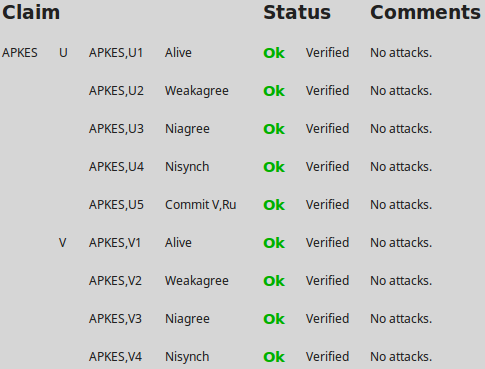
\includegraphics[scale=0.9]{Untitled.png}
	\caption{Results of a verification process using Scyther where all claims are successfully verified.}
	\label{fig:scyther-verify-claims}
\end{figure}


Scyther returns an \texttt{Ok} status code for each claim that is successfully verified. As we see in Figure \ref{fig:scyther-verify-claims}, Scyther is not able to find any attacks on the protocol. To illustrate the case of Scyther actually finding an attack, we try to verify the claims introduced in the section on secrecy, claiming that \texttt{Ru} and \texttt{Rv} are secret. In our example protocol, both nonces are sent in plaintext between U and V, hence this claim will naturally fail as seen in Figure \ref{fig:scyther-verify-claims-fail}.

\begin{figure}[h]
	\centering
	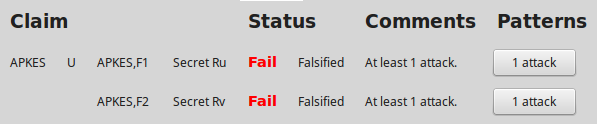
\includegraphics[scale=0.81]{ScytherFailSecretClaim.png}
	\caption{Results of a verification process using Scyther when a claim fails.}
	\label{fig:scyther-verify-claims-fail}
\end{figure}

Whenever Scyther finds an attack on a protocol, it will also provide a concrete description of the attack as graph. An example of such a graph is shown in Figure \ref{fig:scyther-graph}. It contains description of the different runs that Scyther executes, and shows how an adversary can pass messages a cross different runs to learn some secret information for constructing its attack.

\begin{figure}[h]
	\centering
	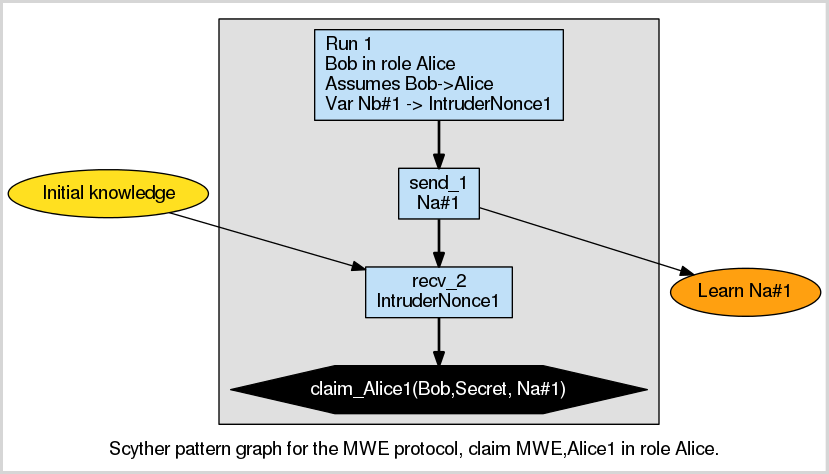
\includegraphics[scale=0.45]{ScytherFailAttackGraph.png}
	\caption{When Scyther finds an attack on a protocol, if will also provide a graph of the attack.}
	\label{fig:scyther-graph}
\end{figure}


\chapter{6LoWPAN Security - Adding Compromise Resilience to the 802.15.4 Security Sublayer}
\label{chp:krentz-6lowpan}


\section{Ideas of the Paper}

APKES. Threeway handshake.

\section{Informal Analysis}

...

\section{Formal Analysis}

\subsection{Scyther}


Script. Explanations. Compare.







%\chapter{TBA}

%\chapter{Conclusion}


%\chapter{Appendix}

\renewcommand*{\bibname}{References}
\bibliographystyle{chicago}
\bibliography{main}

%% Uncomment the following if you have any appendix
% \appendix
% \addtocontents{toc}{%
%  \protect\vspace{1em}% 
%  \protect\noindent \bfseries \appendixtocname\protect\par
%  \protect\vspace{-.5em}%
% }
% \renewcommand{\chaptername}{\appendixname}
%% include below possible appendices (chapters)


\end{document} 
